\documentclass[11pt]{article}
\usepackage[margin=1in]{geometry}
\usepackage{amsmath,amssymb}
\usepackage{graphicx}
\usepackage{booktabs}
\usepackage{subcaption}
\usepackage[hidelinks]{hyperref}
\usepackage{enumitem}
\setlist{nosep,leftmargin=*}
\graphicspath{{figures/}}

\title{CS 771 Homework 3: DDPM and Rectified Flow \\ with U-Net and ViT}
\author{Aditya Kumar \quad Amogh Dixit \quad Shivam Mittal}
\date{}

\begin{document}
\maketitle
\vspace{-2em}

\paragraph{Contributions.} 
Aditya implemented the U-Net decoder and the DDPM loss and sampler, ran the two MNIST DDPM experiments and ran the FID evaluations.
Amogh implemented the ViT forward pass and the rectified flow loss and sampler, ran the two MNIST FM experiments and set up the Colab training pipeline.
Shivam implemented latent modeling for DDPM and FM, ran the two MiniImageNet experiments and implemented and evaluated classifier-free guidance.
Each member wrote the report sections for their own parts, and all three reviewed the full report.

\paragraph{Setup.} We used the supplied configurations without changes. MNIST runs used an NVIDIA A100 and MiniImageNet runs used an NVIDIA L4, both on Google Colab. No packages beyond \texttt{requirements.txt} are needed. Outside the four required files, we only added three command line flags to \texttt{eval.py} (\texttt{-{}-no-cfg}, \texttt{-{}-cfg-scale}, \texttt{-{}-cfg-start-t}) that override \texttt{test\_cfg} for the CFG study. All required FID numbers use \texttt{-{}-no-cfg}.

\section{Prediction Networks}

\paragraph{U-Net decoder.} The U-Net \cite{ronneberger2015unet} follows the conditional design of Stable Diffusion \cite{rombach2022ldm}. The decoder mirrors the encoder. Each decoder level (1) concatenates the current features with the saved encoder output of the same resolution (popped from the list, so the deepest level comes first), (2) applies a ResBlock that maps the doubled channels back down, (3) applies a SpatialTransformer if that level has attention, and (4) upsamples if it is not the last level. A final GroupNorm, SiLU and $1\times1$ convolution give the output.

\emph{Time.} The timestep goes through a sinusoidal embedding and an MLP. Every ResBlock projects this vector to its channel count and adds it to the feature map after the first convolution. This is a per-channel shift, so every layer at every resolution knows the noise level.

\emph{Class.} The label goes through an embedding table and an MLP to form a single context token. The SpatialTransformer blocks use cross-attention with image features as queries and this token as key and value. This injects class information at the attention levels and in the middle block.

\paragraph{ViT (LightningDiT) forward pass.} The ViT \cite{dosovitskiy2021vit} is LightningDiT \cite{yao2025lightningdit}, a DiT \cite{peebles2023dit} with RoPE, QK-norm, RMSNorm and SwiGLU. After patch embedding and position embedding (supplied), we form one conditioning vector $c = e_t + e_y$ from the time and label embeddings. Each DiT block takes the tokens and $c$. The final layer maps each token to a $p\times p\times C$ patch, and \texttt{unpatchify} rebuilds the image.

\emph{Time and class.} Both enter only through $c$, using adaptive LayerNorm (adaLN-Zero) \cite{peebles2023dit}. In each block, an MLP on $c$ predicts a shift, scale and gate for the attention branch and for the MLP branch. These modulate every token in the same way, so time and class control global feature statistics instead of being extra tokens. The modulation layers start at zero, so each block starts as the identity, which makes training stable.

\section{DDPM}
We follow the DDPM paper \cite{ho2020ddpm}.
\paragraph{Loss.} For each image we sample $t \sim \mathcal{U}\{0,\dots,T-1\}$ and $\epsilon \sim \mathcal{N}(0,I)$, build $x_t = \sqrt{\bar\alpha_t}\,x_0 + \sqrt{1-\bar\alpha_t}\,\epsilon$ with \texttt{q\_sample}, and minimize $\|\epsilon - \epsilon_\theta(x_t, c, t)\|^2$ (Algorithm 1).

\paragraph{Reverse step and sampling.} \texttt{p\_sample} computes the mean from Eq.~11,
\[
\mu_\theta = \frac{1}{\sqrt{\alpha_t}}\Big(x_t - \frac{\beta_t}{\sqrt{1-\bar\alpha_t}}\,\epsilon_\theta(x_t,c,t)\Big),
\]
and returns $\mu_\theta + \sigma_t z$ with $z\sim\mathcal{N}(0,I)$ and $\sigma_t^2$ set to the supplied posterior variance. At the last step ($t=0$) it returns the mean with no added noise. \texttt{generate} starts from Gaussian noise and calls \texttt{p\_sample} for $t = T-1$ down to $0$ (Algorithm 2), then postprocesses to $[0,1]$.

\section{Rectified Flow}
We follow rectified flow \cite{liu2023rf} and the flow matching guide \cite{lipman2024fmguide}.
\paragraph{Loss.} We sample noise $z\sim\mathcal{N}(0,I)$ and $t\sim\mathcal{U}[0,1]$, build $x_t = (1-t)z + t\,x_{\text{data}}$, and regress the network output onto $x_{\text{data}} - z$ with MSE.
\emph{Path:} the straight line between noise and data. It is the simplest path and has a constant velocity, so the target is easy to compute.
\emph{Target:} the velocity $x_{\text{data}} - z$, the derivative of the path.
\emph{Time distribution:} uniform on $[0,1]$. It weights all parts of the path equally and is the simplest baseline. Other choices, such as logit-normal sampling, put more weight on the middle of the path \cite{esser2024sd3}. The raw $t\in[0,1]$ is passed to the network, as in SiT \cite{ma2024sit}, which matches the range used at sampling time.

\paragraph{Sampling.} We start from $y_0\sim\mathcal{N}(0,I)$ and apply forward Euler, $y_{t+\Delta t} = y_t + \Delta t\, f_\theta(y_t, c, t)$, with $\Delta t = 1/T$ and $t = 0, \Delta t, \dots, 1-\Delta t$. No noise is added after initialization.

\section{MNIST Results}

\begin{figure}[!htbp]
\centering
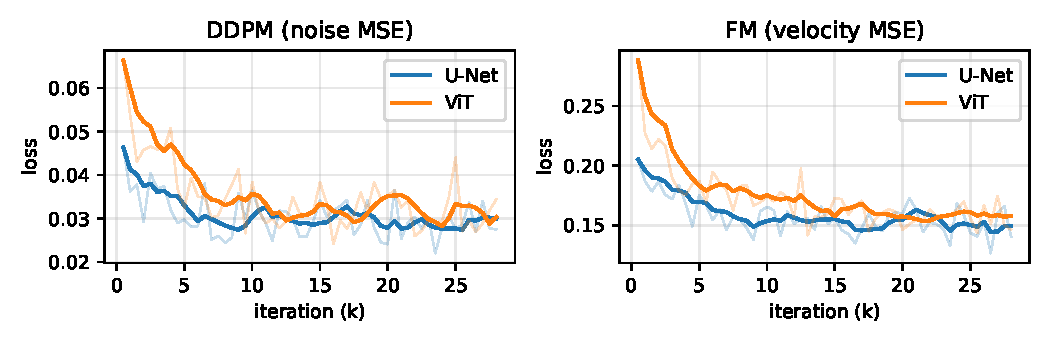
\includegraphics[width=0.9\textwidth]{mnist_curves.pdf}
\vspace{-0.8em}
\caption{MNIST training loss (faint: logged value every 500 iterations, solid: moving average). The two panels use different targets, so their scales are not comparable.}
\label{fig:mnist_curves}
\end{figure}

\begin{figure}[!htbp]
\centering
\begin{subfigure}{0.24\textwidth}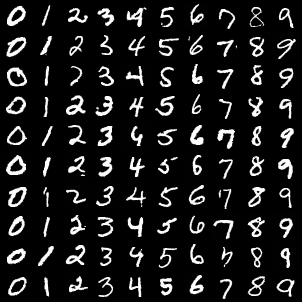
\includegraphics[width=\linewidth]{mnist_ddpm_unet.png}\caption{DDPM U-Net}\end{subfigure}
\begin{subfigure}{0.24\textwidth}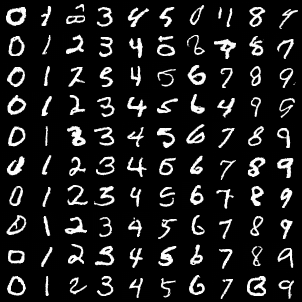
\includegraphics[width=\linewidth]{mnist_ddpm_vit.png}\caption{DDPM ViT}\end{subfigure}
\begin{subfigure}{0.24\textwidth}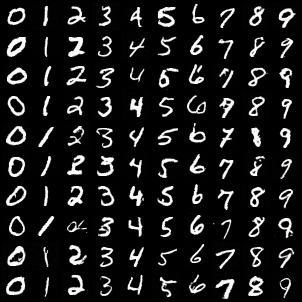
\includegraphics[width=\linewidth]{mnist_fm_unet.png}\caption{FM U-Net}\end{subfigure}
\begin{subfigure}{0.24\textwidth}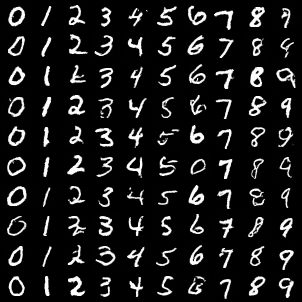
\includegraphics[width=\linewidth]{mnist_fm_vit.png}\caption{FM ViT}\end{subfigure}
\vspace{-0.5em}
\caption{MNIST samples from the final EMA models (epoch 29). Each column is one class, 0 to 9.}
\label{fig:mnist_samples}
\end{figure}

\begin{table}[!htbp]
\centering
\small
\begin{tabular}{lccccc}
\toprule
Model & Backbone & Params & Sampling steps (NFE) & Train time (A100) & FID $\downarrow$ \\
\midrule
DDPM & U-Net & 7.46M & 500 & 0.84 h & \textbf{8.19} \\
DDPM & ViT   & 5.50M & 500 & 0.63 h & 10.16 \\
FM   & U-Net & 7.46M & 10  & 0.74 h & 14.01 \\
FM   & ViT   & 5.50M & 10  & 0.77 h & 12.08 \\
\bottomrule
\end{tabular}
\caption{MNIST \cite{lecun1998mnist} results (30 epochs, 1,000 generated images, FID \cite{heusel2017fid} against the test split). Train time is wall-clock time from the logs, including periodic sample grids and checkpoints.}
\label{tab:mnist}
\end{table}

\paragraph{Discussion.} All four models learn the task. The losses drop quickly in the first 5k iterations and then flatten (Fig.~\ref{fig:mnist_curves}), and every grid shows readable digits in the correct column (Fig.~\ref{fig:mnist_samples}).
\emph{Backbones:} the U-Net starts at a lower loss and converges faster in both settings. Its convolutions give a strong local prior, while the ViT must learn spatial structure from patches and its zero-initialized adaLN layers make it start slowly. The final quality is close. The U-Net is better for DDPM (8.19 vs 10.16) and the ViT is better for FM (12.08 vs 14.01), with about 26\% fewer parameters. The DDPM ViT grid has a few malformed or wrong-class digits.
\emph{FM vs DDPM:} DDPM gives the best FID, but it needs 500 network evaluations per image. FM uses only 10 Euler steps, so sampling is 50$\times$ cheaper, at the cost of 2 to 6 FID points. FM digits have slightly rougher strokes and faint background specks, which is expected from a coarse 10-step ODE solve. FM could use more steps at test time without retraining if better quality is needed.

\section{Latent Modeling and MiniImageNet}

\paragraph{Implementation.} When \texttt{use\_vae} is on, the data loader keeps images in $[0,1]$. In \texttt{compute\_loss} of both DDPM and FM, we encode the batch with the frozen TAESD \cite{taesd} encoder under \texttt{torch.no\_grad()} and apply the same loss to the latents. The model constructor already sets the network input shape to the latent shape, and the VAE weights are frozen. In \texttt{generate}, we sample in latent space and decode with the TAESD decoder at the end, then clamp to $[0,1]$.

\paragraph{Latent vs pixel space.} As in latent diffusion \cite{rombach2022ldm}, a $3\times128\times128$ MiniImageNet \cite{vinyals2016miniimagenet} image becomes a $4\times16\times16$ latent, 48$\times$ fewer values. The network works on a much smaller tensor (64 tokens for the ViT instead of 4,096), which makes training at $128\times128$ affordable. The model learns the distribution of compressed features instead of pixels, and the autoencoder handles fine detail. This also means quality is capped by the autoencoder, and the loss is measured in latent space, not pixel space. The extra cost is one encoder pass per training batch and one decoder pass per sample.

\begin{figure}[!htbp]
\centering
\begin{minipage}{0.42\textwidth}
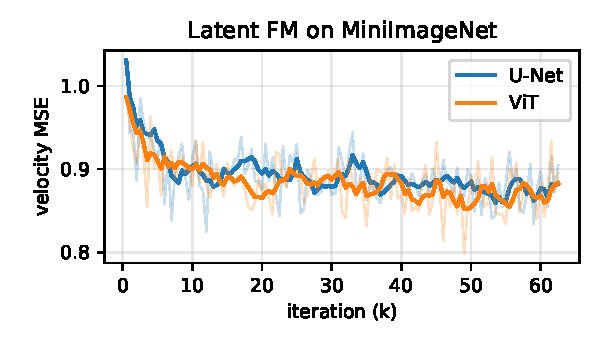
\includegraphics[width=\linewidth]{mini_curves.pdf}
\end{minipage}\hfill
\begin{minipage}{0.55\textwidth}
\small
\centering
\begin{tabular}{lcc}
\toprule
 & U-Net & ViT \\
\midrule
Parameters & 16.77M & 18.35M \\
Train time (L4, 80 epochs) & 1.95 h & 2.38 h \\
Time per iteration & 0.11 s & 0.14 s \\
Sampling steps (NFE) & 10 & 10 \\
FID $\downarrow$ (no CFG) & 119.1 & \textbf{115.1} \\
\bottomrule
\end{tabular}
\end{minipage}
\caption{Latent FM on MiniImageNet. Left: training loss. Right: cost and final FID of the EMA checkpoints (5,000 generated images, 50 per class).}
\label{fig:mini}
\end{figure}

\begin{figure}[!htbp]
\centering
\begin{subfigure}{0.495\textwidth}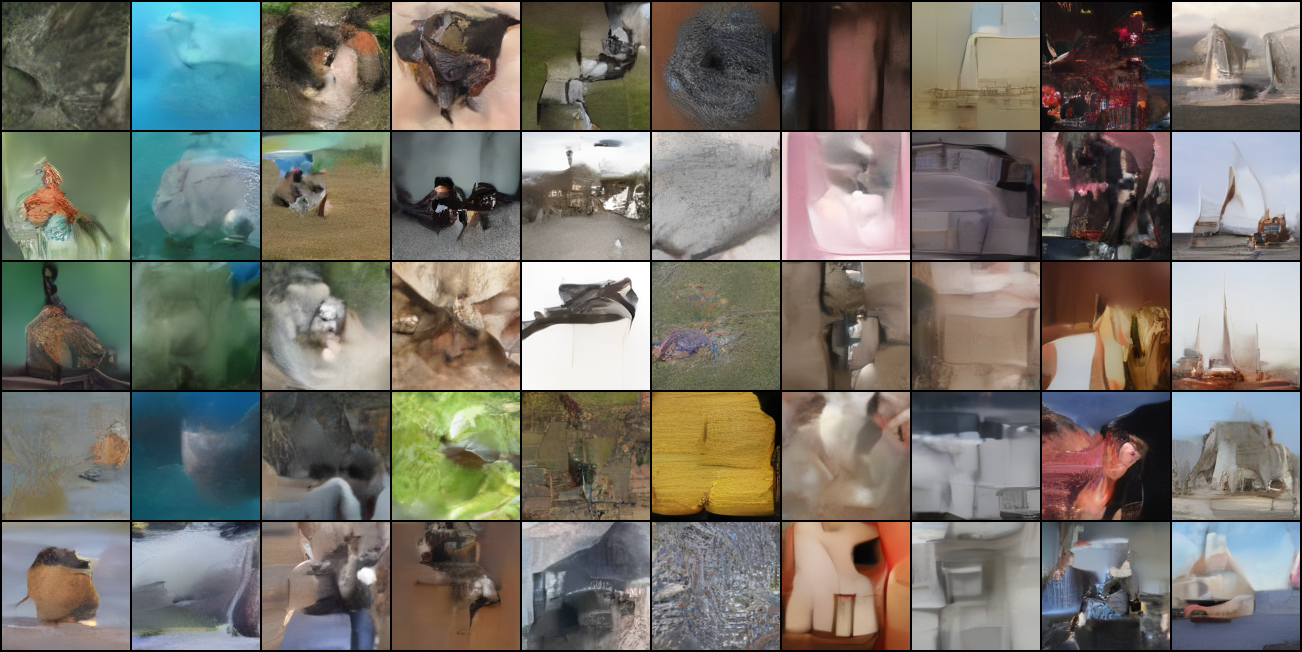
\includegraphics[width=\linewidth]{miniimagenet_fm_unet_ep79.png}\caption{U-Net}\end{subfigure}\hfill
\begin{subfigure}{0.495\textwidth}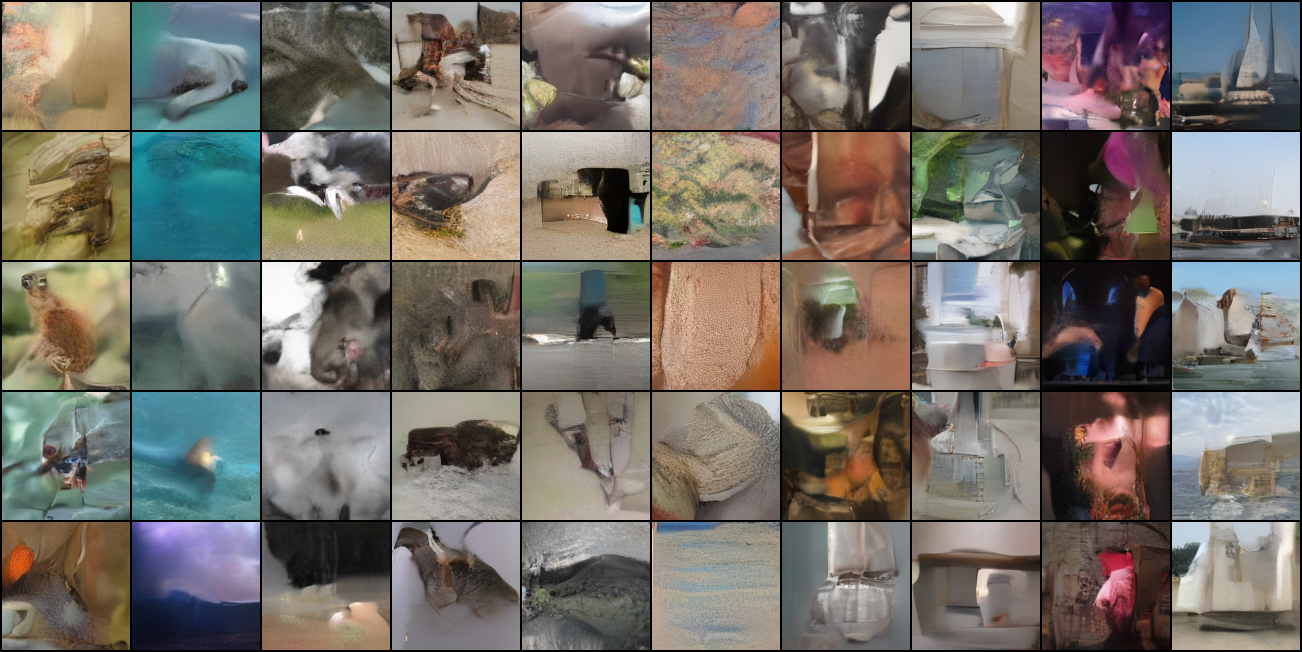
\includegraphics[width=\linewidth]{miniimagenet_fm_vit_ep79.png}\caption{ViT}\end{subfigure}
\vspace{-0.5em}
\caption{MiniImageNet samples from the final EMA models without CFG. Each column is one class (every 10th of the 100 classes).}
\label{fig:mini_samples}
\end{figure}

\paragraph{Discussion.} Both models train stably (Fig.~\ref{fig:mini}). The loss falls fast in the first few thousand iterations and then decreases slowly. It stays near 0.88 because the velocity target includes the random noise, which cannot be predicted.
\emph{Quality:} the ViT is slightly better (FID 115.1 vs 119.1). In Fig.~\ref{fig:mini_samples}, both models produce class-consistent colors, textures and scenes (for example, sailing ships on water in the last column of both grids), but clear objects are rare. This matches the small training budget.
\emph{Cost:} the ViT has 9\% more parameters and took 22\% longer to train. Sampling cost is the same for both (10 network evaluations plus one decode). Training on MiniImageNet took about 2 to 2.5 h per model, compared with under 1 h for MNIST, even with the latent compression.

\section{Bonus: Classifier-Free Guidance}

\paragraph{Implementation.} We implement CFG \cite{ho2022cfg} for both DDPM and FM. The supplied label embedder already replaces the label with a null class (index \texttt{num\_classes}) with probability 0.1 during training, so the same network learns both conditional and unconditional predictions. At sampling time we run the conditional and null-label inputs in one batch and combine them as
\[
\hat f = f_\theta(x, \varnothing, t) + s\,\big(f_\theta(x, c, t) - f_\theta(x, \varnothing, t)\big),
\]
where $f$ is the noise for DDPM and the velocity for FM. Guidance is applied only after the sampling progress (0 at noise, 1 at the image) passes \texttt{cfg\_start\_t} $=0.1$, so the first FM step is unguided. Each guided step costs two network evaluations. No retraining is needed.

\begin{table}[!htbp]
\centering
\small
\begin{tabular}{lcccc}
\toprule
Backbone & No CFG & $s=1.5$ & $s=2.5$ & $s=4.0$ \\
\midrule
U-Net & 119.1 & 102.4 & 79.4 & 66.9 \\
ViT   & 115.1 & 98.6 & 72.3 & \textbf{57.9} \\
\bottomrule
\end{tabular}
\caption{MiniImageNet FID with CFG (same checkpoints and evaluation settings as Fig.~\ref{fig:mini}).}
\label{tab:cfg}
\end{table}

\begin{figure}[!htbp]
\centering
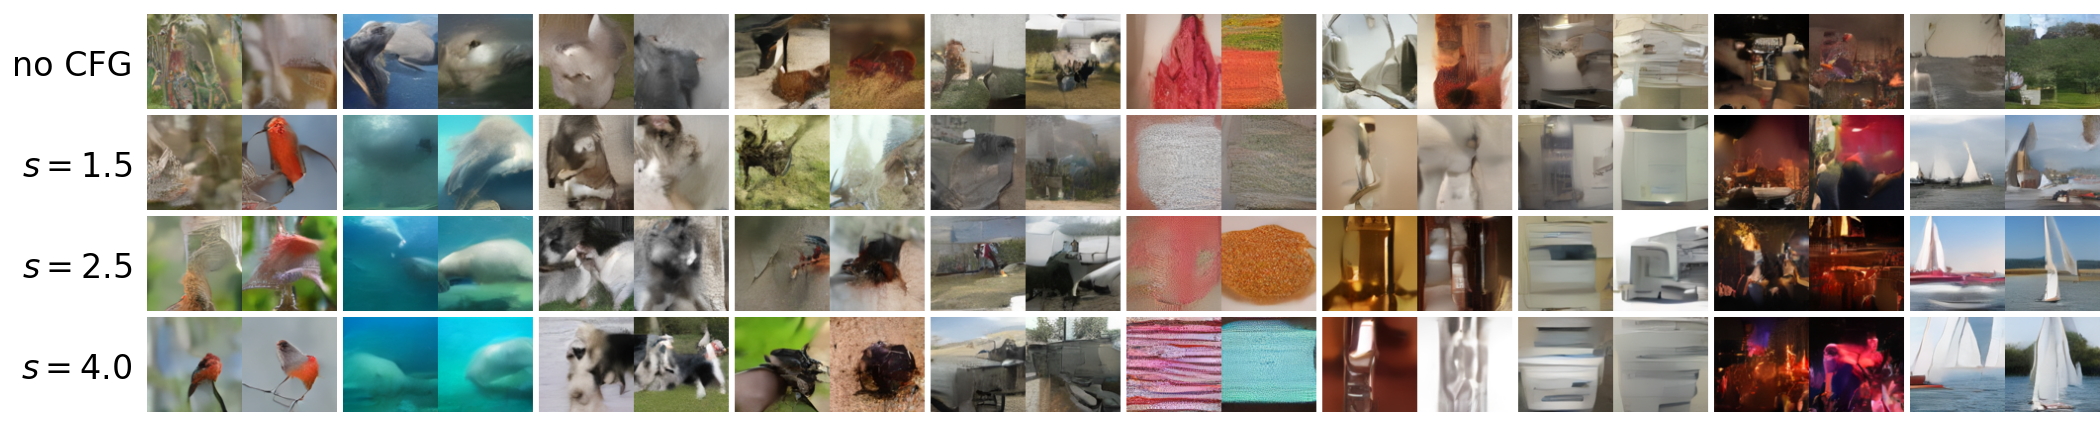
\includegraphics[width=\textwidth]{cfg_vit.png}
\vspace{-1.5em}
\caption{ViT samples with increasing guidance scale. Each pair of columns is one class (every 10th class), with two samples per class. Rows use different random noise. The U-Net shows the same trend (see \texttt{results/}).}
\label{fig:cfg}
\end{figure}

\paragraph{Discussion.} CFG gives a large gain at no training cost (Table~\ref{tab:cfg}). FID improves steadily with the scale, and at $s=4$ it drops by 44\% for the U-Net and 50\% for the ViT. The ViT benefits more and stays ahead at every scale.
\emph{Quality and class adherence:} without CFG, many samples do not show their class and look like blurry mixtures of textures (Fig.~\ref{fig:cfg}). As $s$ grows, objects become sharper and clearly class specific, for example red birds in the first class and sailboats in the last class at $s=4$. Guidance moves each update further in the direction that separates the class from the unconditional prediction, so samples commit to one class instead of averaging over many.
\emph{Diversity:} diversity drops as $s$ grows. At $s=4$, samples of the same class share pose, color and background (the two sailboat samples are nearly the same scene), and colors become more saturated. FID penalizes low diversity, so a very large scale would eventually make FID worse. We did not reach that point within $s\le4$, so at this training budget the gain in fidelity outweighs the loss in diversity. The cost is $2\times$ network evaluations per guided step.

\small
\begin{thebibliography}{99}
\setlength{\itemsep}{0pt}

\bibitem{dosovitskiy2021vit} A.~Dosovitskiy, L.~Beyer, A.~Kolesnikov, D.~Weissenborn, X.~Zhai, T.~Unterthiner, M.~Dehghani, M.~Minderer, G.~Heigold, S.~Gelly, et al. An image is worth 16x16 words: Transformers for image recognition at scale. In \emph{ICLR}, 2021.

\bibitem{esser2024sd3} P.~Esser, S.~Kulal, A.~Blattmann, R.~Entezari, J.~M\"uller, H.~Saini, Y.~Levi, D.~Lorenz, A.~Sauer, F.~Boesel, et al. Scaling rectified flow transformers for high-resolution image synthesis. In \emph{ICML}, 2024.

\bibitem{heusel2017fid} M.~Heusel, H.~Ramsauer, T.~Unterthiner, B.~Nessler, and S.~Hochreiter. GANs trained by a two time-scale update rule converge to a local Nash equilibrium. In \emph{NeurIPS}, 2017.

\bibitem{ho2020ddpm} J.~Ho, A.~Jain, and P.~Abbeel. Denoising diffusion probabilistic models. In \emph{NeurIPS}, 2020.

\bibitem{ho2022cfg} J.~Ho and T.~Salimans. Classifier-free diffusion guidance. \emph{arXiv preprint arXiv:2207.12598}, 2022.

\bibitem{lecun1998mnist} Y.~LeCun, L.~Bottou, Y.~Bengio, and P.~Haffner. Gradient-based learning applied to document recognition. \emph{Proceedings of the IEEE}, 86(11):2278--2324, 1998.

\bibitem{lipman2024fmguide} Y.~Lipman, M.~Havasi, P.~Holderrieth, N.~Shaul, M.~Le, B.~Karrer, R.~T.~Q.~Chen, D.~Lopez-Paz, H.~Ben-Hamu, and I.~Gat. Flow matching guide and code. \emph{arXiv preprint arXiv:2412.06264}, 2024.

\bibitem{liu2023rf} X.~Liu, C.~Gong, and Q.~Liu. Flow straight and fast: Learning to generate and transfer data with rectified flow. In \emph{ICLR}, 2023.

\bibitem{ma2024sit} N.~Ma, M.~Goldstein, M.~S.~Albergo, N.~M.~Boffi, E.~Vanden-Eijnden, and S.~Xie. SiT: Exploring flow and diffusion-based generative models with scalable interpolant transformers. In \emph{ECCV}, 2024.

\bibitem{peebles2023dit} W.~Peebles and S.~Xie. Scalable diffusion models with transformers. In \emph{ICCV}, 2023.

\bibitem{rombach2022ldm} R.~Rombach, A.~Blattmann, D.~Lorenz, P.~Esser, and B.~Ommer. High-resolution image synthesis with latent diffusion models. In \emph{CVPR}, 2022.

\bibitem{ronneberger2015unet} O.~Ronneberger, P.~Fischer, and T.~Brox. U-Net: Convolutional networks for biomedical image segmentation. In \emph{MICCAI}, 2015.

\bibitem{taesd} Tiny autoencoder for Stable Diffusion (TAESD). \url{https://github.com/madebyollin/taesd}, 2022.

\bibitem{vinyals2016miniimagenet} O.~Vinyals, C.~Blundell, T.~Lillicrap, K.~Kavukcuoglu, and D.~Wierstra. Matching networks for one shot learning. In \emph{NeurIPS}, 2016.

\bibitem{yao2025lightningdit} J.~Yao, B.~Yang, and X.~Wang. Reconstruction vs.\ generation: Taming optimization dilemma in latent diffusion models. In \emph{CVPR}, 2025.

\end{thebibliography}

\end{document}
